%%%%%%%%%%%%%%%%%%%%%%%%%%%%%%%%%%%%%%%%%%%%%%%%%%%%%%%%%%%%%%%%%%%%%%%%%%%%
%% Trim Size: 9.75in x 6.5in
%% Text Area: 8in (include Runningheads) x 5in
%% ws-ijitdm.tex  :  8-7-2009 
%% Class file to use with ws-ijitdm.cls written in Latex2E. 
%% The content, structure, format and layout of this style file is the 
%% property of World Scientific Publishing Co. Pte. Ltd. 
%% Copyright 1995, 2002 by World Scientific Publishing Co. 
%% All rights are reserved.
%%%%%%%%%%%%%%%%%%%%%%%%%%%%%%%%%%%%%%%%%%%%%%%%%%%%%%%%%%%%%%%%%%%%%%%%%%%%

\documentclass{ws-ijitdm}

\begin{document}

\markboth{Authors' Names}
{Instructions for Typing Manuscripts (Paper's Title)}

\catchline{0}{0}{0000}{}{}

\title{INSTRUCTIONS FOR TYPESETTING MANUSCRIPTS\\
USING \TeX\ OR \LaTeX\footnote{\uc{F}or the title, try 
not to use more than 3 lines.
\uc{T}ypeset the title in 10 pt roman, uppercase and
boldface.}
}

\author{\footnotesize FIRST AUTHOR\footnote{
\uc{T}ypeset names in 8 pt roman, uppercase. \uc{U}se the footnote to 
indicate the present or permanent address of the author.}}

\address{University Department, University Name, Address\\
City, State ZIP/Zone,
Country\footnote{\uc{S}tate completely without abbreviations, the
affiliation and mailing address, including country. \uc{T}ypeset in 8 pt
italic.}
}

\author{SECOND AUTHOR}

\address{Group, Laboratory, Address\\
City, State ZIP/Zone, Country
}

\maketitle

\begin{history}
\received{Day Month Year}
\revised{Day Month Year}
\end{history}

\begin{abstract}
The abstract should summarize the context, content
and conclusions of the paper in less than 200 words. It should
not contain any references or displayed equations. Typeset the
abstract in 8 pt roman with baselineskip of 10 pt, making
an indentation of 1.5 pica on the left and right margins.

\keywords{Keyword1; keyword2; keyword3.}
\end{abstract}

\section{General Appearance}	

Contributions to {\it International Journal of Information Technology
\& Decision}\break 
{\it Making} are to be in American English. Authors are
encouraged to have their contribution checked for grammar. American
spelling should be used. Abbreviations are allowed but should be spelt
out in full when first used. Integers ten and below are to be spelt
out.  Italicize foreign language phrases (e.g.~Latin, French).  Upon
acceptance, authors are required to submit their data source file
including postscript files for figures.

The text is to be typeset in 10 pt roman, single spaced with
baselineskip of 13~pt. Text area (including copyright block) 
is 8 inches high and 5 inches wide for the first page.  Text area
(excluding running title) is 7.7 inches high and 5 inches wide for
subsequent pages.  Final pagination and insertion of running titles
will be done by the publisher.

\section{Running Heads}

Please provide a shortened running head (not more than eight words) for
the title of your paper. This will appear on the top right-hand side
of your paper.

\section{Major Headings}

Major headings should be typeset in boldface with the first
letter of important words capitalized.

\subsection{Sub-headings}

Sub-headings should be typeset in boldface italic and capitalize
the first letter of the first word only. Section number to be in
boldface roman.

\subsubsection{Sub-subheadings}

Typeset sub-subheadings in medium face italic and capitalize the
first letter of the first word only. Section numbers to be in
roman.

\subsection{Numbering and spacing}

Sections, sub-sections and sub-subsections are numbered in
Arabic.  Use double spacing before all section headings, and
single spacing after section headings. Flush left all paragraphs
that follow after section headings.

\subsection{Lists of items}

Lists may be laid out with each item marked by a dot:
\begin{itemlist}
 \item item one,
 \item item two.
\end{itemlist}
Items may also be numbered in lowercase roman numerals:
\begin{romanlist}[(ii)]
\item item one
\item item two 
\begin{romanlist}[(b)]
\item Lists within lists can be numbered with lowercase roman letters,
\item second item. 
\end{romanlist}
\end{romanlist}

\section{Equations}

Displayed equations should be numbered consecutively in each
section, with the number set flush right and enclosed in
parentheses

\renewcommand{\theequation}{\thesection.\arabic{equation}}
\setcounter{equation}{0}
\begin{equation}
\mu(n, t) = \frac{\sum^\infty_{i=1} 1(d_i < t, N(d_i) = n)}{
\int^t_{\sigma=0} 1(N(\sigma) = n)d\sigma}\,.
\label{diseqn}
\end{equation}

Equations should be referred to in abbreviated form,
e.g.~``Eq.~(\ref{diseqn})'' or ``(\ref{diseqn})''. In multiple-line
equations, the number should be given on the last line.

Displayed equations are to be centered on the page width.
Standard English letters like x are to appear as $x$
(italicized) in the text if they are used as mathematical
symbols. Punctuation marks are used at the end of equations as
if they appeared directly in the text.

\section{Theorem Environments}

\begin{theorem}
Theorems, lemmas, etc. are to be numbered
consecutively in the paper. Use double spacing before and after
theorems, lemmas, etc.
\end{theorem}

\begin{proof}
Proofs should end with
\end{proof}

\section{Illustrations and Photographs}

Figures are to be inserted in the text nearest their first
reference.  Original india ink drawings of glossy prints are
preferred. Please send one set of originals with 
copies. If the author requires the publisher to reduce the figures, 
ensure that the figures (including letterings and numbers) are large
enough to be clearly seen after reduction. If photographs are to be
used, only black and white ones are acceptable.

\begin{figure}[th]
\centerline{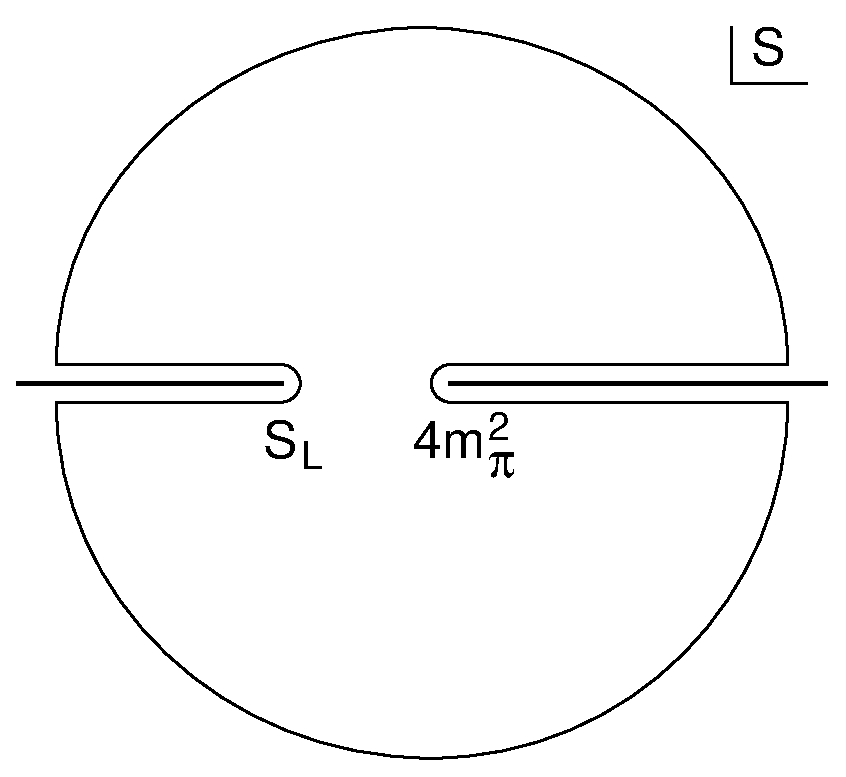
\psfig{file=ijitdmf1.eps,width=4.9cm}}
\vspace*{8pt}
\caption{A schematic illustration of dissociative recombination. The
direct mechanism, 4m$^2_\pi$ is initiated when the
molecular ion S$_{\rm L}$ captures an electron with kinetic energy.}
\end{figure}


Figures are to be placed either top or bottom and 
sequentially numbered in Arabic numerals. The
caption must be placed below the figure. Typeset in 8 pt
roman with baselineskip of 10~pt. Use double spacing between a
caption and the text that follows immediately.

Previously published material must be accompanied by written
permission from the author and publisher.

\section{Tables}

Tables should be inserted in the text as close to the point of
reference as possible. Some space should be left above and below
the table.

\begin{table}[ph]
\tbl{Comparison of acoustic for frequencies for piston-cylinder problem.}
{\begin{tabular}{@{}cccc@{}} \toprule
Piston mass & Analytical frequency & TRIA6-$S_1$ model &
\% Error \\
& (Rad/s) & (Rad/s) \\ \colrule
1.0\hphantom{00} & \hphantom{0}281.0 & \hphantom{0}280.81 & 0.07 \\
0.1\hphantom{00} & \hphantom{0}876.0 & \hphantom{0}875.74 & 0.03 \\
0.01\hphantom{0} & 2441.0 & 2441.0\hphantom{0} & 0.0\hphantom{0} \\
0.001 & 4130.0 & 4129.3\hphantom{0} & 0.16\\ \botrule
\end{tabular}}
\end{table}

Tables should be numbered sequentially in the text in Arabic
numerals. Captions are to be centralized above the tables.
Typeset tables and captions in 8 pt roman with baselineskip of 10 pt.

If tables need to extend over to a second page, the continuation
of the table should be preceded by a caption, 
e.g.~``{\it Table 2.} $(${\it Continued}$)$''

\section{Footnotes}

Footnotes should be numbered sequentially in superscript
lowercase roman letters.\footnote{Footnotes should be
typeset in 8 pt roman at the bottom of the page.}

\section*{Acknowledgments}

This section should come before the References. Dedications and funding 
information may also be included here.

\appendix

\section{Appendices}

Appendices should be used only when absolutely necessary. They
should come after the References. If there is more than one
appendix, number them alphabetically. Number displayed equations
occurring in the Appendix in this way, e.g.~(\ref{appeqn}), (A.2),
etc.
\begin{equation}
\mu(n, t) = {\sum^\infty_{i=1} 1(d_i < t, N(d_i) = n)}{
\int^t_{\sigma=0} 1(N(\sigma) = n)d\sigma}\,.
\label{appeqn}
\end{equation}

\section*{References}

References are to be listed in the order cited in the text in Arabic
numerals.  They can be typed in superscripts after punctuation marks,
e.g.~``$\ldots$ in the statement.\cite{1}'' or used directly,
e.g.~``see Ref.~5 for examples.'' Please list using the style shown in
the following examples.  For journal names, use the standard
abbreviations or spell in full. Typeset references in 9 pt roman.

\begin{thebibliography}{00}
\bibitem{1} C. M. Wang, J. N. Reddy and K. H. Lee, {\it Shear Deformable  
Beams} (Elsevier, Oxford, 2000).
	
\bibitem{2} R. Loren and D. B. Benson, {\it Introduction to String Field
Theory}, 2nd edn. (Springer-Verlag, New York, 1999).  

\bibitem{3} C. M. Wang (ed.), {\it Shear Deformable Beams} 
(Elsevier, Oxford, 2000).  

\bibitem{4} R. Loren and D. B. Benson (eds.), {\it Introduction to 
String Field Theory}, 2nd edn. (Springer-Verlag, New York, 1999).  

\bibitem{5} C. M. Wang, J. N. Reddy and K. H. Lee, New set of buckling
parameters, in {\it Shear Deformable Beams}, ed.~T. Rex 
(Elsevier, Oxford, 2000), pp.~201--213.

\bibitem{6} R. Loren, J. Li and D. B. Benson, Deterministic flow-chart 
interpretations, in {\it Introduction to String Field Theory}, 
eds.~J. Randy and K. Tan (Springer-Verlag, New York, 1999), p.~400.

\bibitem{7} R. Loren, J. Li and D. B. Benson, Deterministic 
flow-chart interpretations, in {\it Introduction to String Field Theory},  
Advanced Series in Mathematical Physics, Vol.~3 
(Springer-Verlag, New York, 1999), pp.~401--413.  

\bibitem{8} R. Loren, J. Li and D. B. Benson, Deterministic flow-chart 
interpretations, in {\it Proc. 3rd Int. Conf. Entity-Relationship 
Approach}, eds.~C. G. Davis and R. T. Yeh (North-Holland, Amsterdam, 1983), 
pp.421--439.

\bibitem{9} R. Loren and D. B. Benson, Deterministic flow-chart 
interpretations, {\it J. Comput. System Sci}. {\bf 27}(2, Suppl. 290) 
(1983) 400--433.

\bibitem{10} B. Lee, String field theory, {\it J. Comput. System Sci}. 
{\bf 27}(1983) 400--433, doi:10.1142/S0219199703001026.  

\bibitem{11} R. Loren, Foundations of resource development, 
{\it D-lib Magazine} (1999), http://www.dlib.org/jul99/07loren.html.

\bibitem{12} B. Lee, String field theory, {\it J. Comput. System Sci}. 
{\bf 27}(1983) 400--433, doi:10.1142/S0219199703001026.

\end{thebibliography}

\end{document}


